平壁面镜像法和圆定理

使用如下记号,对于复函数$f(z)$,记$\bar{f}(z)$为对$f$中除$z$以外的复数取共轭。如果$f(z)$描述了原无界流场中的复势,
则在$x$轴加一固壁后,得到新的满足固壁条件的复势为:
\begin{equation}\label{eq:101xAdd}
w(z)=f(z)+\bar{f}(z)
\end{equation}

可以用奇点叠加法来理解\eqref{eq:101xAdd}式,为简单起见我们只考虑$f(z)$是由基本解叠加的情形,即原流场有若干个点源、点汇、点涡,偶极子
\begin{equation}\label{eq:101xAdd}
f(z)=\sum_{k} a_k \ln(z-z_k)+ \frac{b_k}{z-z_k}
\end{equation}
其中$a_k=\frac{Q_k+i\Gamma_k}{2\pi},b_k=\frac{-M}{2\pi}$
如果我们把这些奇点的位置关于$x$轴镜像,注意到点涡在镜像过程中旋转方向反向,即$\Gamma_k$变为$-\Gamma_k$,
偶极子的朝向也镜像过程中也发生反向,
相当于$M=me^{i\beta}$变成了$me^{-i\beta}$,可以验证镜像场和原场的叠加场在$x$处复势虚部为零,
即$x$轴处相当于一条流线,如果把$x$轴换成固壁,将
不会影响原流场的分布,因此做镜像和加固壁对于上半平面产生相同的流场。
%This explanation is not plausiable enough!

% for discussion only
% 如果是$y$轴作为壁面,设在不可压缩平面无旋流动无界域的左半平面上,$z=z_0$处有各阶奇点,它的复势可写作:
% \begin{equation}\label{eq:101z0}
% f(z,z_0)=a_0 \ln(z-z_0)+\sum_{n=1}^N \frac{a_n}{(z-z_0)^n}
% \end{equation}
% 则构造左半平面的复函数
% \begin{equation}\label{eq:101yAdd}
% w(z)=f(z,z_0)+\bar{a}_0 \ln(z+\bar{z}_0)+\sum_{n=1}^N \frac{(-1)^n\bar{a}_n}{(z+\bar{z}_0)^n}
% \end{equation}
% 其中$-\bar{z_0}$为$z_0$关于$y$轴的对称点,
% 无法采用老师课上的写法,式\eqref{eq:101yAdd}简记为:
% $W(z)=f(z)-\bar{f}(z)$。
% 必须讨论n的奇偶性确定是否前面加负号
% 下面说明$W(z)$在$y$轴上虚部为常数,因为有$z=-\bar{z}$,由式\eqref{eq:101yAdd}得
% \begin{align}
% \bar{a}_0 \ln(z+\bar{z}_0)+\sum_{n=1}^N \frac{(-1)^n\bar{a}_n}{(z+\bar{z}_0)^n}=&
% \bar{a}_0 \ln(-\bar{z}+\bar{z}_0)+\sum_{n=1}^N \frac{(-1)^n\bar{a}_n}{(-\bar{z}+\bar{z}_0)^n}\\
% =&\bar{a}_0 (\ln(\bar{z}-\bar{z}_0)+\ln(-1))+\sum_{n=1}^N \frac{\bar{a}_n}{(\bar{z}-\bar{z}_0)^n}\\
% =&\bar{f}(\bar{z},\bar{z}_0)+\bar{a}_0\pi i
% \end{align}
% 因此式\eqref{eq:101yAdd}的虚部为$\Real(a_0)\pi$为常数。
% 所以$w(z)$是$y$轴作壁面的复势。
% It can be seen that Teacher is right...
如果是$y$轴作为壁面,可以直接验证$f(z)+\bar{f}(-z)$在$y$轴上的虚部为零,因此可作为左半平面的复势。

如果加入的是一圆柱壁面,复平面方程为$zz^*=a^2$。则圆定理指出,加入圆柱壁面后复势为$w(z)=f(z)+\bar{f}(\frac{a^2}{z})$,
可以直接验证$w(z)$在壁面上虚部为零。

若原流场为均匀流$uz$,加圆柱壁面后复势为$w(z)=uz+u\frac{a^2}{z}$,即为圆柱绕流的复势,与
\eqref{eq:92PotentialAroundCylinder}式给出的复势无环量的情形相同。

对柱面外一点涡,$f(z)=\frac{\Gamma}{2\pi i}\ln(z-z_0)$,则加圆柱壁面后复势(去掉一些常数)为
\begin{equation}
w(z)=\frac{\Gamma}{2\pi i}\ln(z-z_0)+\frac{\Gamma}{2\pi i}\ln(z)-\frac{\Gamma}{2\pi i}\ln(z-\frac{a^2}{z_0})
\end{equation}
该复势由壁面外$z_0$外一逆时针点涡和壁面内原点处逆时针点涡、$\frac{a^2}{z_0}$处顺时针点涡叠加而成,如图
\ref{fig:pointVortexImage}所示。
\begin{figure}[!ht]
 \centering
 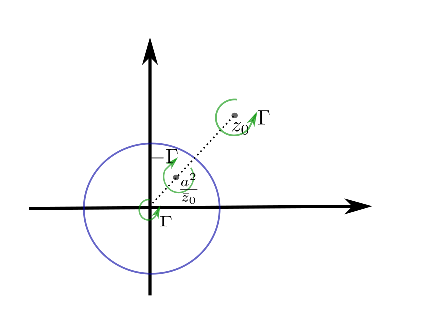
\includegraphics[width=8cm]{pointVortexImage.eps}
 \caption{柱面外一点涡等效于三个点涡叠加产生的复势}\label{fig:pointVortexImage}
\end{figure}
%库塔-儒科夫斯基环量条件 用到保角映射,自学需花时间,跳过-^-

黏性流体力学

黏性流体力学使用雷诺数(Reynold Number)来表征流体的特征,当$\Rey<\Rey_{c1}$时流动的主要特征表现为层流(Laminar flow);
当$\Rey>\Rey_{c2}$时流动的主要特征表现为湍流(Turbulent flow)。当雷诺数$\Rey$在下临界雷诺数$\Rey_{c1}$和上临界雷诺数
之间$\Rey_{c2}$时由于扰动的存在层流和湍流可能会相互转化。

雷诺数定义为:
\begin{equation}
\Rey=\frac{UL}{v}
\end{equation}
\begin{itemize}
\item $U$:流动的特征速度
\item $L$:流动的特征长度
\item $v$:运动黏性系数
\end{itemize}

雷诺数的物理意义为惯性力和黏性力量级之比,当$\Rey >>1$时,可忽略黏性,采用理想流体模型;
当$\Rey <<1 $时,可忽略惯性,当作极慢运动处理。
%\begin{equation}
%\end{equation}
